\section{Metodología utilizada}


\subsection{Base de datos utilizada}

\vspace{5 mm}

A continuación hablaremos sobre la base de datos que hemos utilizado, los inconvenientes que hemos encontrado al usarla y como los hemos solucionado.

La base de datos que hemos usado se llama \textbf{Vietnamese Foods} y la subío un estudiante de la VNU HCMC a la web \textbf{kaggle}. Este dataset consta de 24474 imágenes divididas en 29 clases. Las imágenes no fueron previamente divididas en un set de entrenamiento y un set de test. Tampoco disponíamos de un archivo de texto con la ruta de todas las imágenes del dataset por lo que tuvimos que construirlo a mano usando la orden \textbf{find} que nos proporciona el terminal de Linux.

Una vez obtenido dicho archivo de texto con las imágenes nos fue sencillo construir los correspondientes sets de entrenamiento y test. Tuvimos que cargar todas las imágenes con sus respectivas clases en dos ndarrays, y usarlos en la función \textbf{train\_test\_split} de sklearn con un 0.2 de tamaño de test. Como las clases que usamos eran de tipo string, tuvimos que hacer uso también de la función \textbf{to\_categorical} para convertirlas en valores enteros.

Una vez intentamos cargar las imágenes en memoria nos dimos cuenta que no era posible debido al costo computacional que requería almacenar tantas imágenes en la RAM. Por este motivo redujimos el número de clases de forma aleatoria hasta llegar a \textbf{9}, que era el máximo número de clases que podíamos cargar en Google Colab sin sobrepasar sus recursos computacionales. Hemos decidido tomar esta decisión en lugar de reducir el número de imágenes de cada clase y mantener el número de clases ya que esto generaría una falta de datos a la hora de entrenar cada clase. Cabe destacar que todas las clases del dataset están equilibradas. A continuación mostraré ejemplos de las diferentes imágenes que se pueden encontrar en el dataset usado:

\vspace{5 mm}

\begin{figure}[H]
  \centering
  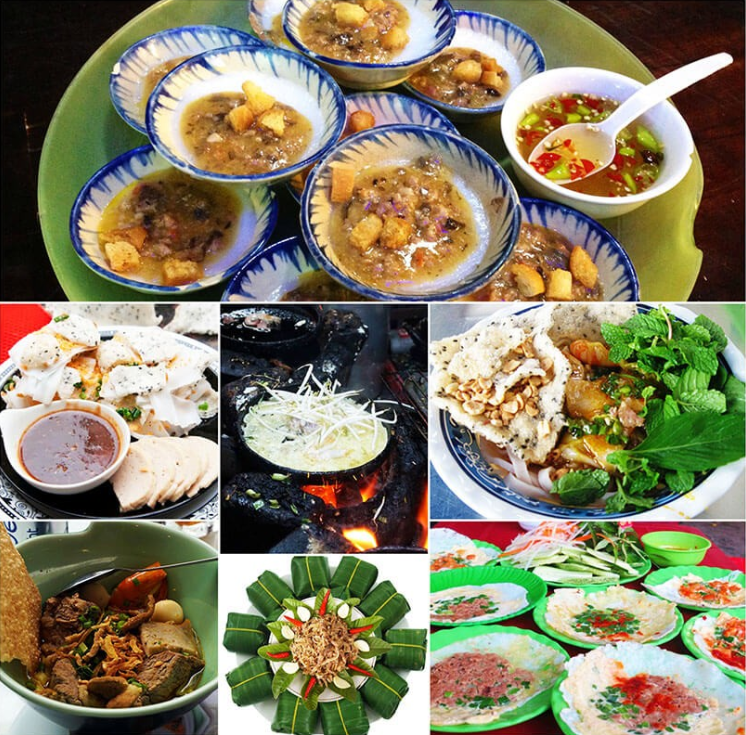
\includegraphics[width=0.5\linewidth]{Imagenes/comida-vietnamita.png}
  \caption{Imágenes del dataset Vietnamese Foods}
  \label{fig:sub-first}
\end{figure}

\newpage

\subsection{Preprocesado de los datos}

Para el preprocesado de los datos a utilizar simplemente hemos utilizado la función de preprocesado de cada red utilizada. Además de esto también hemos redimensionado las imágenes al leerlas de cara a que tengan el mismo tamaño que la entrada de las distintas redes.

También mencionar que este preprocesado se ha aplicado también al conjunto de test a la hora de predecir los valores, como vimos que es necesario tanto en teoría como en la práctica 2.


\subsection{Redes neuronales convolucionales entrenadas con ImageNet utilizadas}

\vspace{5 mm}

En el enunciado del proyecto se nos dice que usemos una red preentrenada en \textbf{ImageNet} de entre un conjunto de redes. Después de analizar los proyectos que hemos incluido en la revisión bibliográfica nos hemos dado cuenta de lo interesante que es analizar el comportamiento de cada red usando la misma base de datos. Es por todo lo anterior que hemos utilizado las siguientes redes neuronales en nuestro proyecto:

\begin{itemize}


\item{\textbf{ResNet-50:}\cite{resnet50} Esta red está compuesta por 48 capas convolucionales junto con 1 capa MaxPooling2D y 1 capa AveragePooling. Tiene un total de 25,636,712 parámetros y una media de 0.749 de Top-1 Accuracy. Se trata de una red muy útil que se usa tanto dentro como fuera de la Visión por Computador.}


\item{\textbf{EfficientNetB0:}\cite{efficientnetb0} Esta red está compuesta por 237 capas divididas en 5 tipos de módulos, donde cada uno de ellos tiene un número de capas diferentes. La red no fue desarrollada por ingenieros, si no por la propia red, la cual utiliza una búsqueda de arquitectura neuronal multiobjetivo que optimiza tanto la precisión como las operaciones de punto flotante. Tiene un total de 5,330,571 parámetros.}

\item{\textbf{DenseNet-121:}\cite{densenet121} Todas las arquitecturas DenseNet están formadas por 4 bloques densos que, dependiendo de la versión que usemos, van a tener diferentes capas en cada uno de esos bloques. Concretamente la versión DenseNet-121 va a tener 6,12,24,16 capas en cada uno de esos bloques respectivamente. Esta versión tiene un total de 8,062,504 parámetros y una media de 0.750 de Top-1 Accuracy.}


\item{\textbf{InceptionV3:}\cite{inceptionv3} Esta red tiene una profundidad de 159 capas. Está compuesta por 11 módulos Inception donde cada módulo consiste en capas MaxPooling2D y capas convolucionales con activación ReLU. Tiene un total de 23,851,784 parámetros y una media de 0.779 de Top-1 Accuracy.}


\end{itemize}

\newpage

\subsection{Mejoras sobre las redes utilizadas}

De cara a mejorar las redes utilizadas hemos realizado distintos experimentos.

Para comenzar, hemos buscado el mejor optimizador posible utilizando una Grid Search, escogiendo finalmente el optimizador Adam, explicado en los fundamentos teoricos de este documento.

Otra de las mejoras introducidas es una ampliación de las redes utilizadas, hemos añadido nuevas capas finales con el objetivo de evitar el sobreajuste de los modelos iniciales, que comentaremos en la sección de resultados, añadiendo capas de dropout y batch normalization.

\begin{lstlisting}
nueva_red = red.output
nueva_red = Dense(1000, activation="relu")(nueva_red)
nueva_red = BatchNormalization(renorm=True)(nueva_red)
nueva_red = Dropout(0.5)(nueva_red)
nueva_red = Dense (NUM_CLASES, activation = 'softmax')(nueva_red)
\end{lstlisting}

También hemos realizado un ajuste fino de la red. Hemos probado tanto a entrenar solo la última capa (capa softmax que sustituye a última capa original y que clasificará la entrada en las clases), y tras eso descongelar la red para hacer el ajuste fino tanto a entrenar las últimas cinco capas más las nuevas capas y tras eso descongelar toda la red y aplicar el ajuste fino.

Ejemplo de crear una red ResNet50 y descongelar las últimas 5 capas.

\begin{lstlisting}
#  celda para el codigo de resnet50, por defecto sin include_top para añadir la capa Dense con nuestro numero de clases y pesos de imagenet
red_resnet = ResNet50(include_top = False, pooling = "avg")
red_resnet.trainable = False
# ponemos los ultimos cinco como entrenables, el resto los fijamos
for layer in red_resnet.layers[-5:]:
  layer.trainable = True
\end{lstlisting}

Por último, y para todos los casos, hemos añadido early stopping de cara a detener el entrenamiento cuando no se logra mejorar el resultado durante cinco épocas, manteniendo los parámetros de la mejor época y no de la última.
